%%%%%%%%%%%%%%%%%%%%%%%%%%%%%%%%%%%%%%%%%%%%%%%%%%%%%%%%%%%%%%%%%%%%%%
% Overleaf (WriteLaTeX) Example: Molecular Chemistry Presentation
%
% Source: http://www.overleaf.com
%
% In these slides we show how Overleaf can be used with standard 
% chemistry packages to easily create professional presentations.
% 
% Feel free to distribute this example, but please keep the referral
% to overleaf.com
% 
%%%%%%%%%%%%%%%%%%%%%%%%%%%%%%%%%%%%%%%%%%%%%%%%%%%%%%%%%%%%%%%%%%%%%%

\documentclass{beamer}

\mode<presentation>
{
  \usetheme{Madrid}       % or try default, Darmstadt, Warsaw, ...
  \usecolortheme{default} % or try albatross, beaver, crane, ...
  \usefonttheme{default}    % or try default, structurebold, ...
  \setbeamertemplate{navigation symbols}{}
  \setbeamertemplate{caption}[numbered]
} 

\usepackage[english]{babel}
\usepackage[utf8x]{inputenc}
\usepackage{chemfig}
\usepackage[version=3]{mhchem}

\usepackage{hyperref}
  \hypersetup{colorlinks=true}
  \hypersetup{urlcolor=blue}
  \hypersetup{linkcolor = .}
\usepackage{xcolor}
\usepackage{siunitx}
  \sisetup{separate-uncertainty = true}
\usepackage{physics}
\usepackage[font=small,labelfont=bf]{caption}
\usepackage{subcaption}
\usepackage[en-GB]{datetime2}
\usepackage{overpic}
\usepackage{feynmp}
\DeclareGraphicsRule{*}{mps}{*}{}

\usepackage{scalerel}
\newcommand{\mylbrace}[2]{\vspace{#2pt}\hspace{6pt}\scaleleftright[\dimexpr5pt+#1\dimexpr0.06pt]{\lbrace}{\rule[\dimexpr2pt-#1\dimexpr0.5pt]{-4pt}{#1pt}}{.}}
\newcommand{\myrbrace}[2]{\vspace{#2pt}\scaleleftright[\dimexpr5pt+#1\dimexpr0.06pt]{.}{\rule[\dimexpr2pt-#1\dimexpr0.5pt]{-4pt}{#1pt}}{\rbrace}\hspace{6pt}}

% Here's where the presentation starts, with the info for the title slide
\title[$B^\pm\to(K^+K^-\pi^+\pi^-)_DK^\pm$]{\texorpdfstring{$\gamma$}{gamma} analysis update in \texorpdfstring{$B^\pm\to(K^+K^-\pi^+\pi^-)_DK^\pm$}{B to K+K-pi+pi-} decays}
\author{Martin Tat}
\institute{Oxford LHCb}
\date{\today}

\titlegraphic{
\includegraphics[height = 3cm, width = 4cm]{lhcb.jpg}\hspace{2cm}~%
              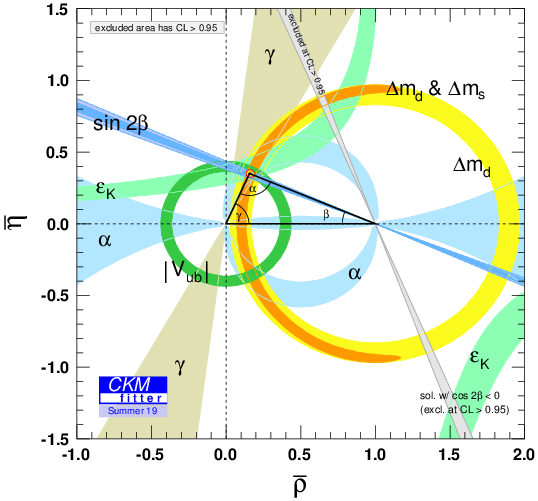
\includegraphics[height = 3cm, width = 4cm]{ckmfitter.png}}

\begin{document}

\begin{frame}
  \titlepage
\end{frame}

% These three lines create an automatically generated table of contents.
\begin{frame}{Outline}
  \tableofcontents
\end{frame}

\section{Summary of last time}
\begin{frame}{Summary of last time}
  \begin{itemize}
    \setlength\itemsep{1.2em}
    \item{$B^\pm\to DK^\pm$, $D\to K^+K^-\pi^+\pi^-$, \href{https://arxiv.org/abs/hep-ph/0611272}{arXiv:hep-ph/0611272}}
    \item{Model independent measurement with BESIII strong phase input}
    \item{Estimate $2000$ $B$ events from LHCb Run $1$ and $2$}
    \begin{itemize}
      \item{Benchmark: $\sigma(\gamma) = \SI{11}{\degree}$ from model dependent fit}
      \item{LHCb amplitude model in AmpGen, \href{https://arxiv.org/abs/1811.08304}{arXiv:1811.08304}}
    \end{itemize}
    \item{Pull study to test and optimize binning scheme}
    \begin{itemize}
      \item{Simulated $1000$ experiments with $2000$ events each}
      \item{Strong phases from amplitude model using MC integration}
    \end{itemize}
  \end{itemize}
\end{frame}

\section{Binning scheme}
\begin{frame}{Binning scheme}
  \begin{itemize}
    \item{Aim: Pick binning scheme to maximize $x_\pm$ and $y_\pm$ sensitivity}
  \end{itemize}
  \begin{block}{Event yield in bin $i$}
    $N^+_i = h_{B^+}\Big(\bar{K_i} + \big(x_+^2 + y_+^2\big)K_i + 2\sqrt{K_i\bar{K_i}}\big(x_+c_i - y_+s_i\big)\Big)$
    $N^+_{-i} = h_{B^+}\Big(K_i + \big(x_+^2 + y_+^2\big)\bar{K_i} + 2\sqrt{K_i\bar{K_i}}\big(x_+c_i + y_+s_i\big)\Big)$
    $x_\pm = r_B\cos(\delta_B\pm\gamma), \quad y_\pm = r_B\sin(\delta_B\pm\gamma)$
  \end{block}
  \begin{itemize}
    \item{Previously: Rectangular parameterization of 5D phase space}
    \item{Better and simpler:}
    \begin{itemize}
      \item{Generate C++ source code for amplitude model using AmpGen}
      \item{Evaluate amplitude directly in analysis}
      \item{Decide bin based on strong phase and amplitude ratio directly}
    \end{itemize}
  \end{itemize}
  \begin{block}{Strong phase and amplitude ratio}
    $\mathcal{A}(D^0)/\mathcal{A}(\bar{D^0}) = r_D\exp(i\delta_D)$
  \end{block}
\end{frame}

\begin{frame}{Naive ampltiude binning scheme}
  \begin{figure}
    \begin{overpic}[scale = 0.19, percent]{Binning1.png}
      \put(24, 34){\huge 1}
      \put(40.5, 34){\huge 2}
      \put(57.5, 34){\huge 3}
      \put(74, 34){\huge 4}
      \put(23, 17){\huge -4}
      \put(39.5, 17){\huge -3}
      \put(56.5, 17){\huge -2}
      \put(73, 17){\huge -1}
    \end{overpic}
  \end{figure}
\end{frame}

\begin{frame}{Pull study naive amplitude binning}
  \begin{figure}
    \centering
    \vspace{-0.2cm}
    \begin{subfigure}{0.5\textwidth}
      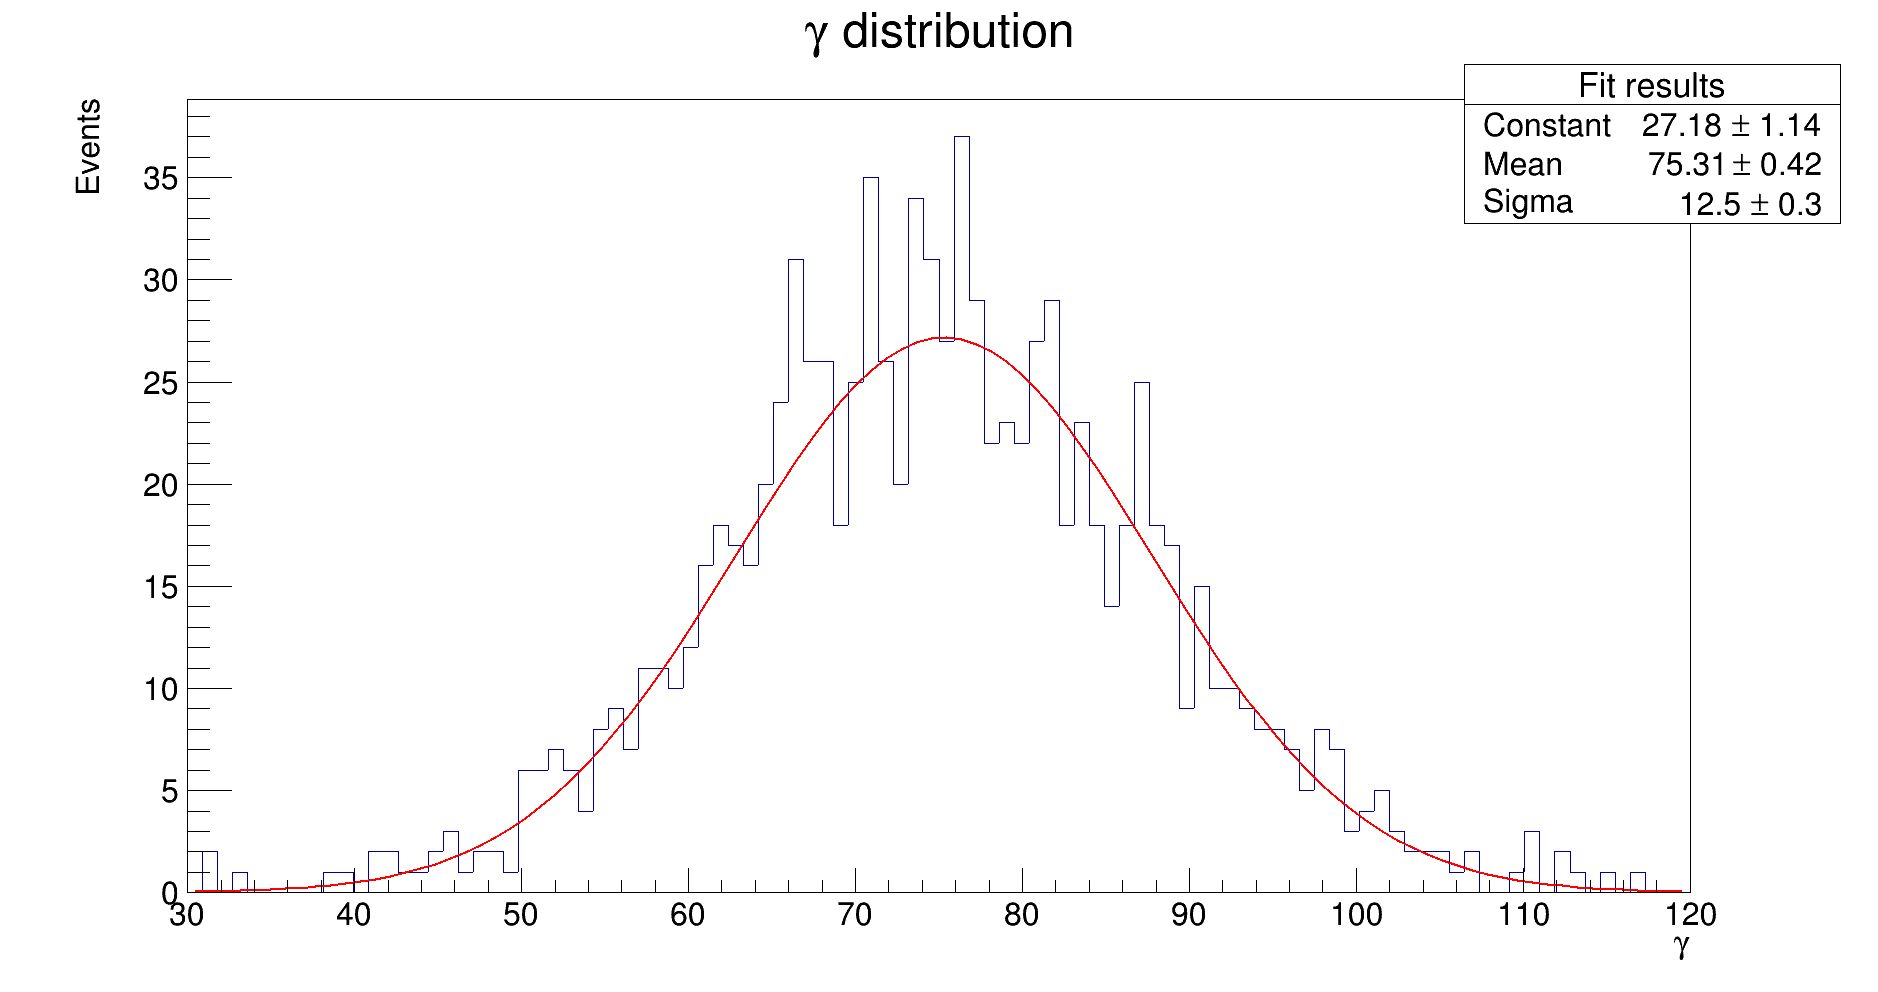
\includegraphics[width = 1.0\textwidth]{GammaDistribution8BinsFixedWidth.png}
      \caption{$\gamma$ distribution}
    \end{subfigure}%
    \begin{subfigure}{0.5\textwidth}
      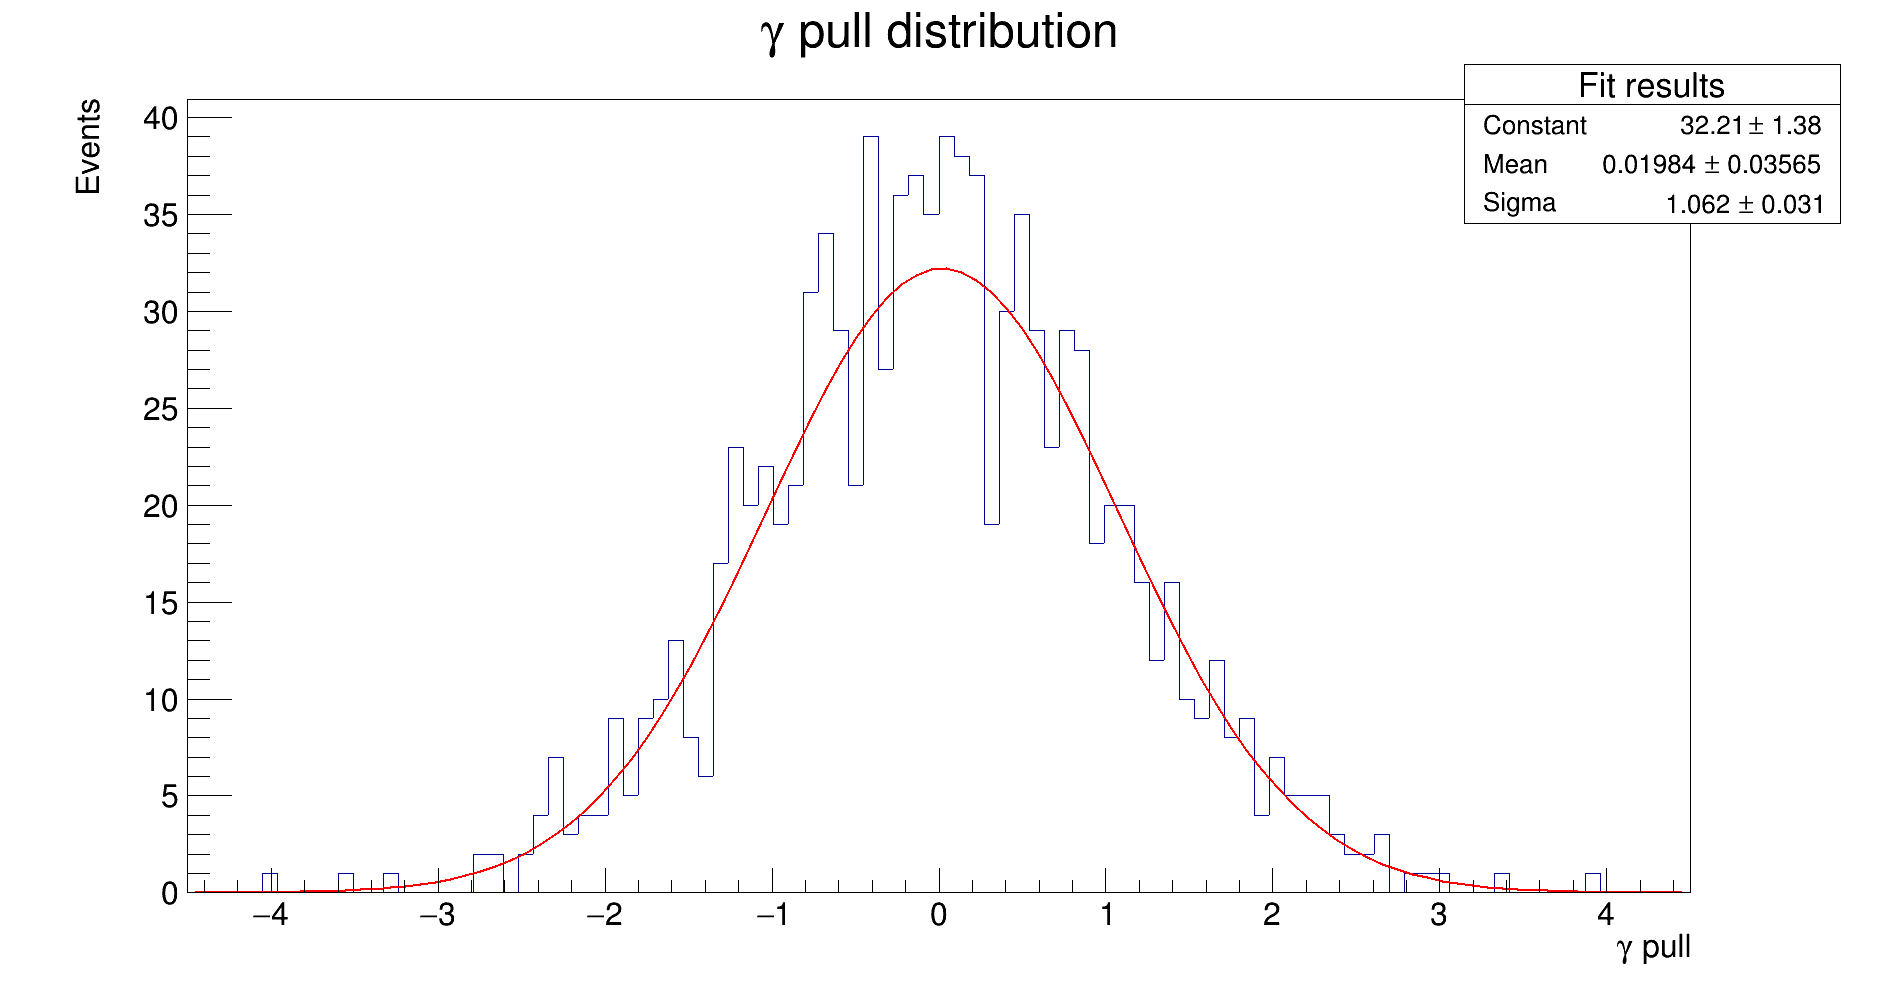
\includegraphics[width = 1.0\textwidth]{GammaPull8BinsFixedWidth.png}
      \caption{$\gamma$ pull}
    \end{subfigure}
  \end{figure}
  \begin{center}
    Achieved $\gamma$ precision of $\sigma(\gamma) = \SI{13}{\degree}$
  \end{center}
\end{frame}

\begin{frame}{Optimize bin widths}
  \begin{itemize}
    \item{Optimize $x_\pm$, $y_\pm$ sensitivity}
    \item{Vary bin edges, keep symmetric around $\delta_D = 0$}
  \end{itemize}
  \begin{block}{Binning $Q$ value}
    $Q^2 = 1 - \sum_i\frac{K_i\bar{K_i}(1 - c_i^2 - s_i^2)}{N_i}\Big/\sum_iK_i$ \\
    $Q^2\approx\sum_iN_i(c_i^2 + s_i^2)\Big/\sum_iN_i$
  \end{block}
  \begin{itemize}
    \item{Can achieve $Q\approx0.90$ with $8$ bins $\implies$ expect $\sigma(\gamma) = \SI{12}{\degree}$}
  \end{itemize}
\end{frame}

\begin{frame}{Variable widths binning scheme}
  \begin{figure}
    \begin{overpic}[scale = 0.19, percent]{Binning3.png}
      \put(26, 34){\huge 1}
      \put(42, 34){\huge 2}
      \put(55, 34){\huge 3}
      \put(72, 34){\huge 4}
      \put(24.5, 17){\huge -4}
      \put(41, 17){\huge -3}
      \put(54, 17){\huge -2}
      \put(70.5, 17){\huge -1}
    \end{overpic}
  \end{figure}
\end{frame}

\begin{frame}{Pull study with variable widths binning}
  \begin{figure}
    \centering
    \vspace{-0.2cm}
    \begin{subfigure}{0.5\textwidth}
      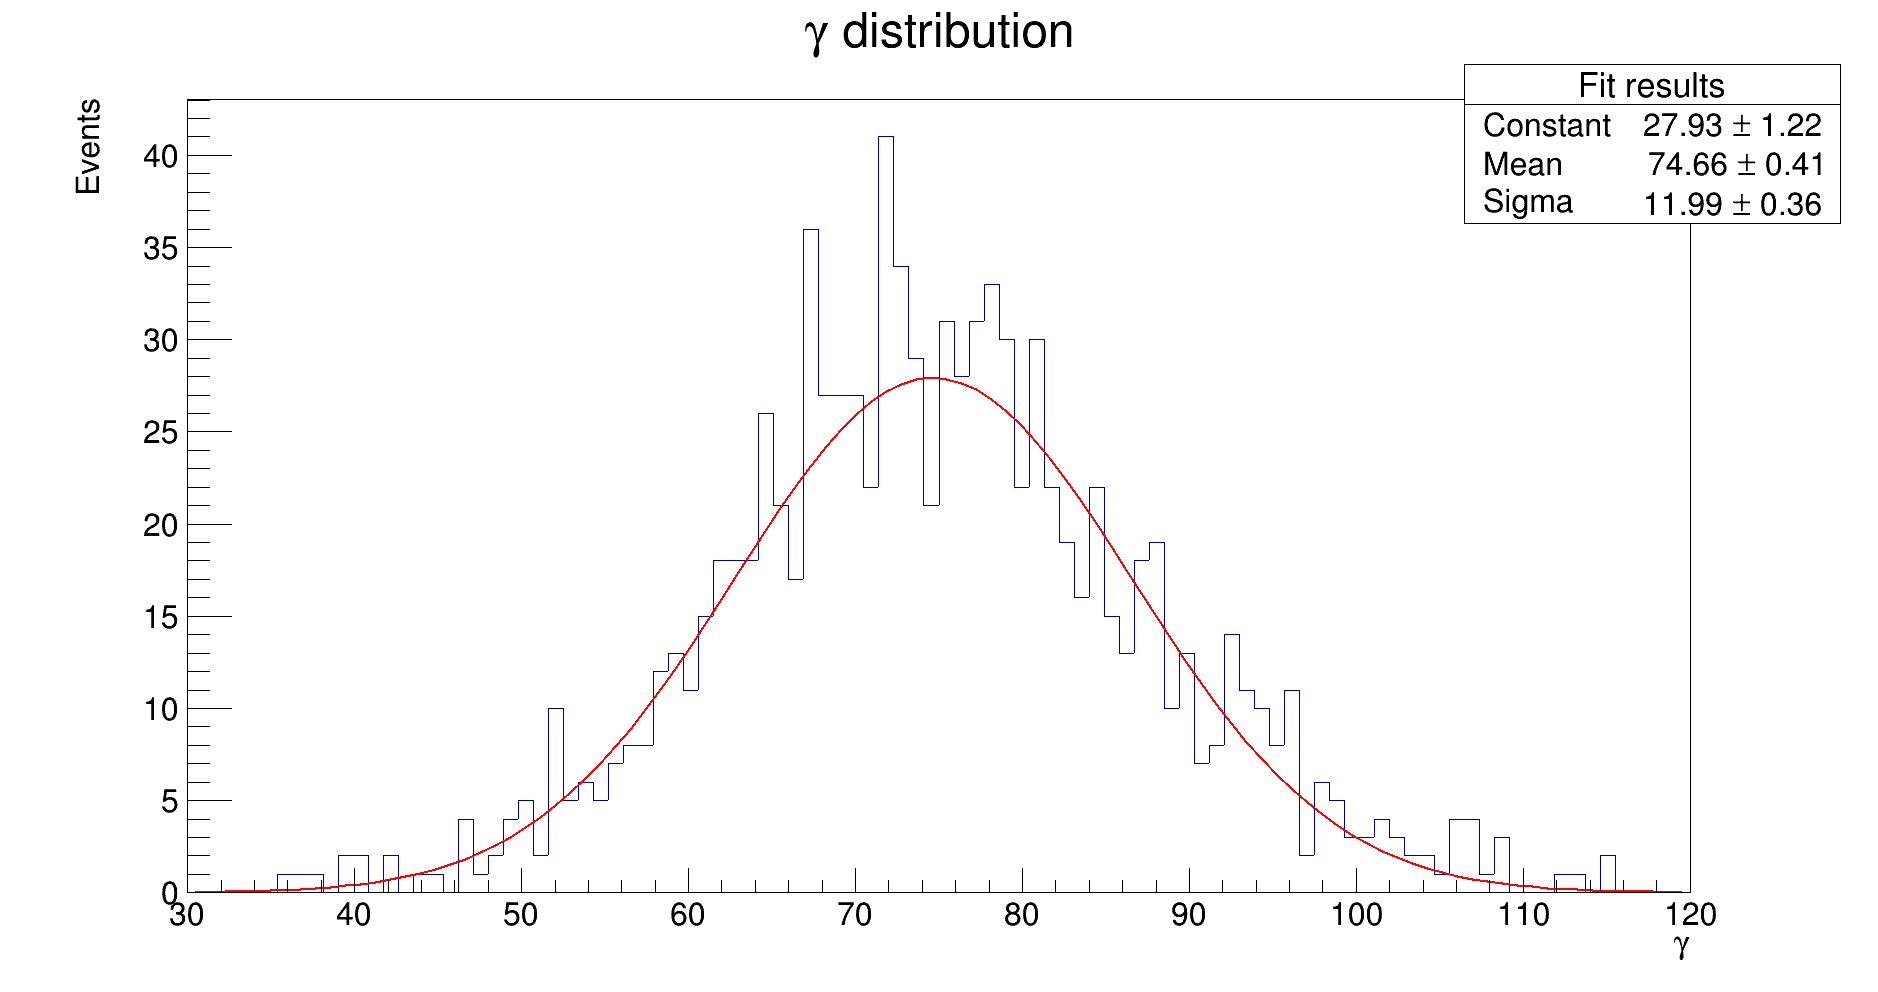
\includegraphics[width = 1.0\textwidth]{GammaDistribution8BinsVariableWidth.png}
      \caption{$\gamma$ distribution}
    \end{subfigure}%
    \begin{subfigure}{0.5\textwidth}
      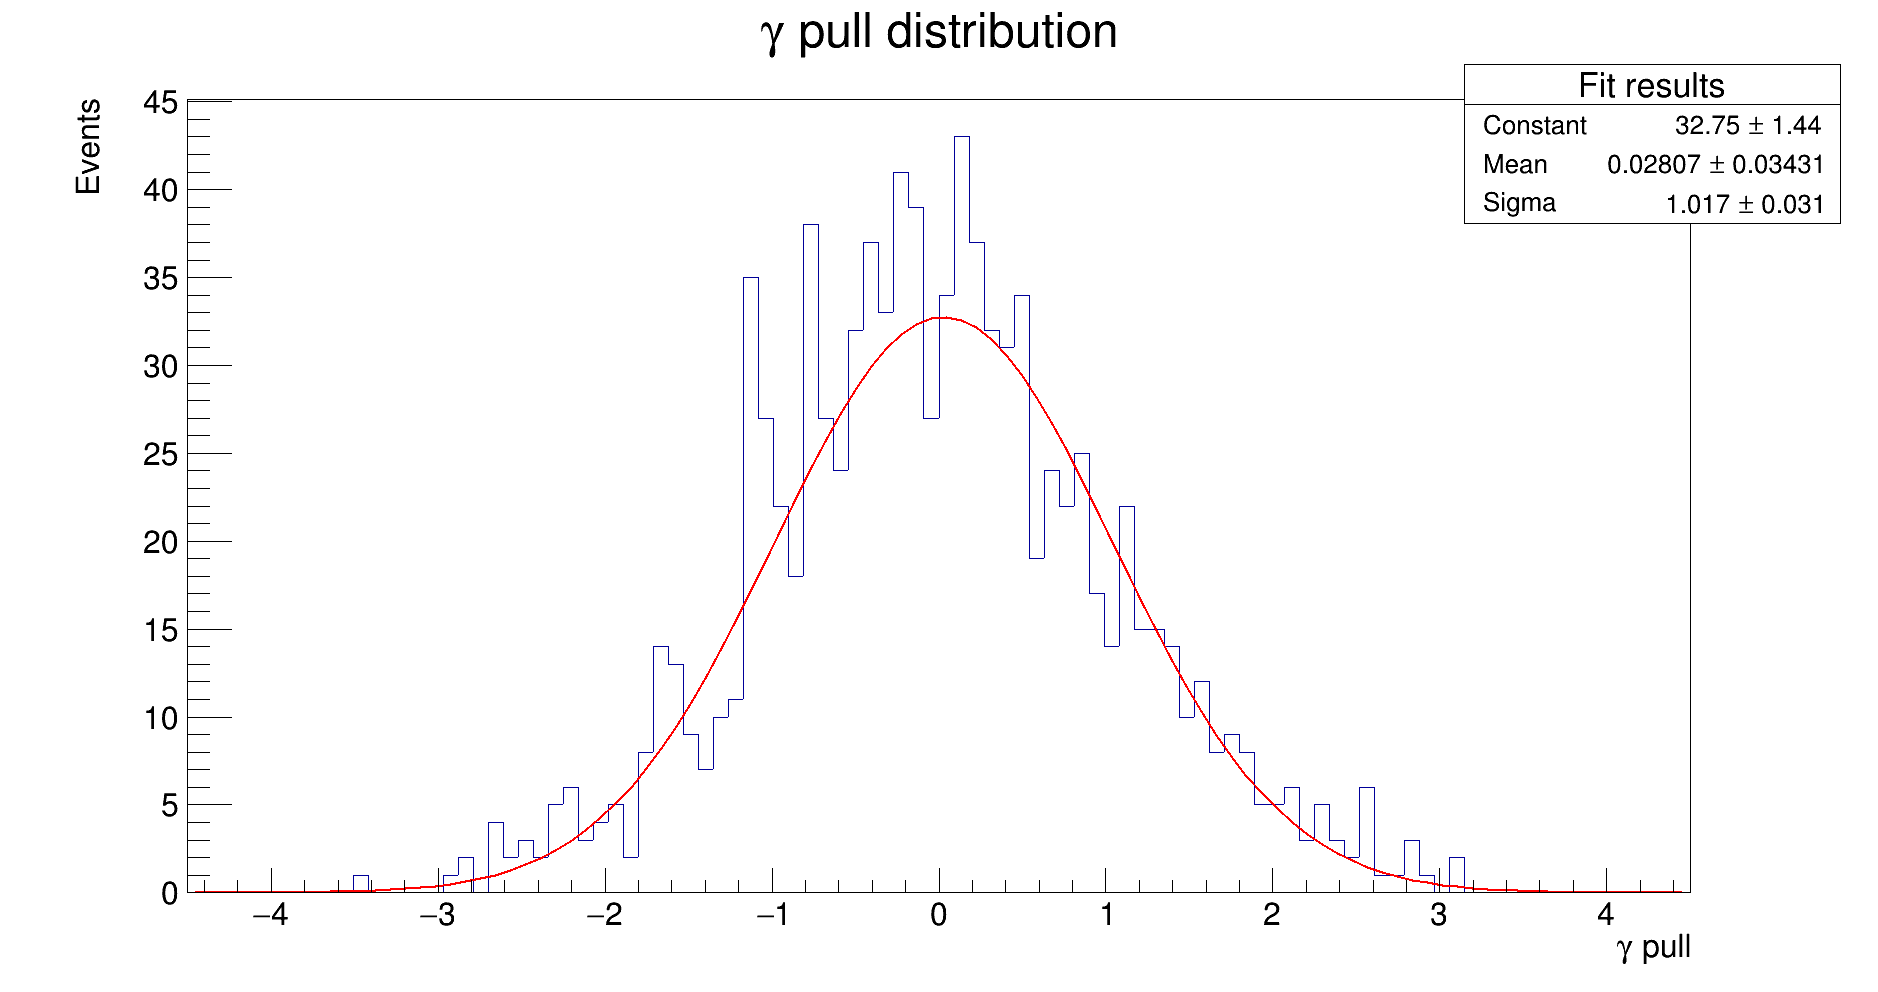
\includegraphics[width = 1.0\textwidth]{GammaPull8BinsVariableWidth.png}
      \caption{$\gamma$ pull}
    \end{subfigure}
  \end{figure}
  \begin{center}
    Achieved $\gamma$ precision of $\sigma(\gamma) = \SI{12}{\degree}$
  \end{center}
\end{frame}

\begin{frame}{Binning along $r_D$}
  \begin{itemize}
    \item{Further optmization by binning along $r_D$}
    \item{Claim: Can use \textbf{same} $c_i$ and $s_i$ in bin $i$ and $i'$}
    \item{Can push $\sigma(\gamma)$ down by $\SI{0.5}{\degree}$-$\SI{1}{\degree}$}
  \end{itemize}
  \begin{figure}
    \vspace{-0.2cm}
    \begin{overpic}[scale = 0.17, percent]{Binning2.png}
      \put(24, 29){\huge 1}
      \put(40.5, 29){\huge 2}
      \put(57.5, 29){\huge 3}
      \put(74, 29){\huge 4}
      \put(24, 38){\huge 1'}
      \put(40.5, 38){\huge 2'}
      \put(57.5, 38){\huge 3'}
      \put(74, 38){\huge 4'}
      \put(23, 20){\huge -4}
      \put(39.5, 20){\huge -3}
      \put(56.5, 20){\huge -2}
      \put(73, 20){\huge -1}
      \put(23, 11){\huge -4'}
      \put(39.5, 11){\huge -3'}
      \put(56.5, 11){\huge -2'}
      \put(73, 11){\huge -1'}
    \end{overpic}
  \end{figure}
\end{frame}

\section{First look at LHCb data}
\begin{frame}{First look at LHCb data}
  \begin{itemize}
    \setlength\itemsep{1.3em}
    \item{DaVinci scripts from $K_S\pi^+\pi^-$ analysis}
    \item{Have obtained full Run $2$ data and MC}
    \item{DaVinci issues with Run $1$, unable to run DecayTreeFitter}
    \item{Event selection:}
    \begin{itemize}
      \item{Initial rectangular cuts}
      \item{Gradient Boosted Decision Tree}
      \item{Final cuts}
      \item{Mass fit}
    \end{itemize}
  \end{itemize}
\end{frame}

\begin{frame}{First look at LHCb data}
  \begin{figure}
    \centering
    \vspace{-0.2cm}
    \begin{subfigure}{0.5\textwidth}
      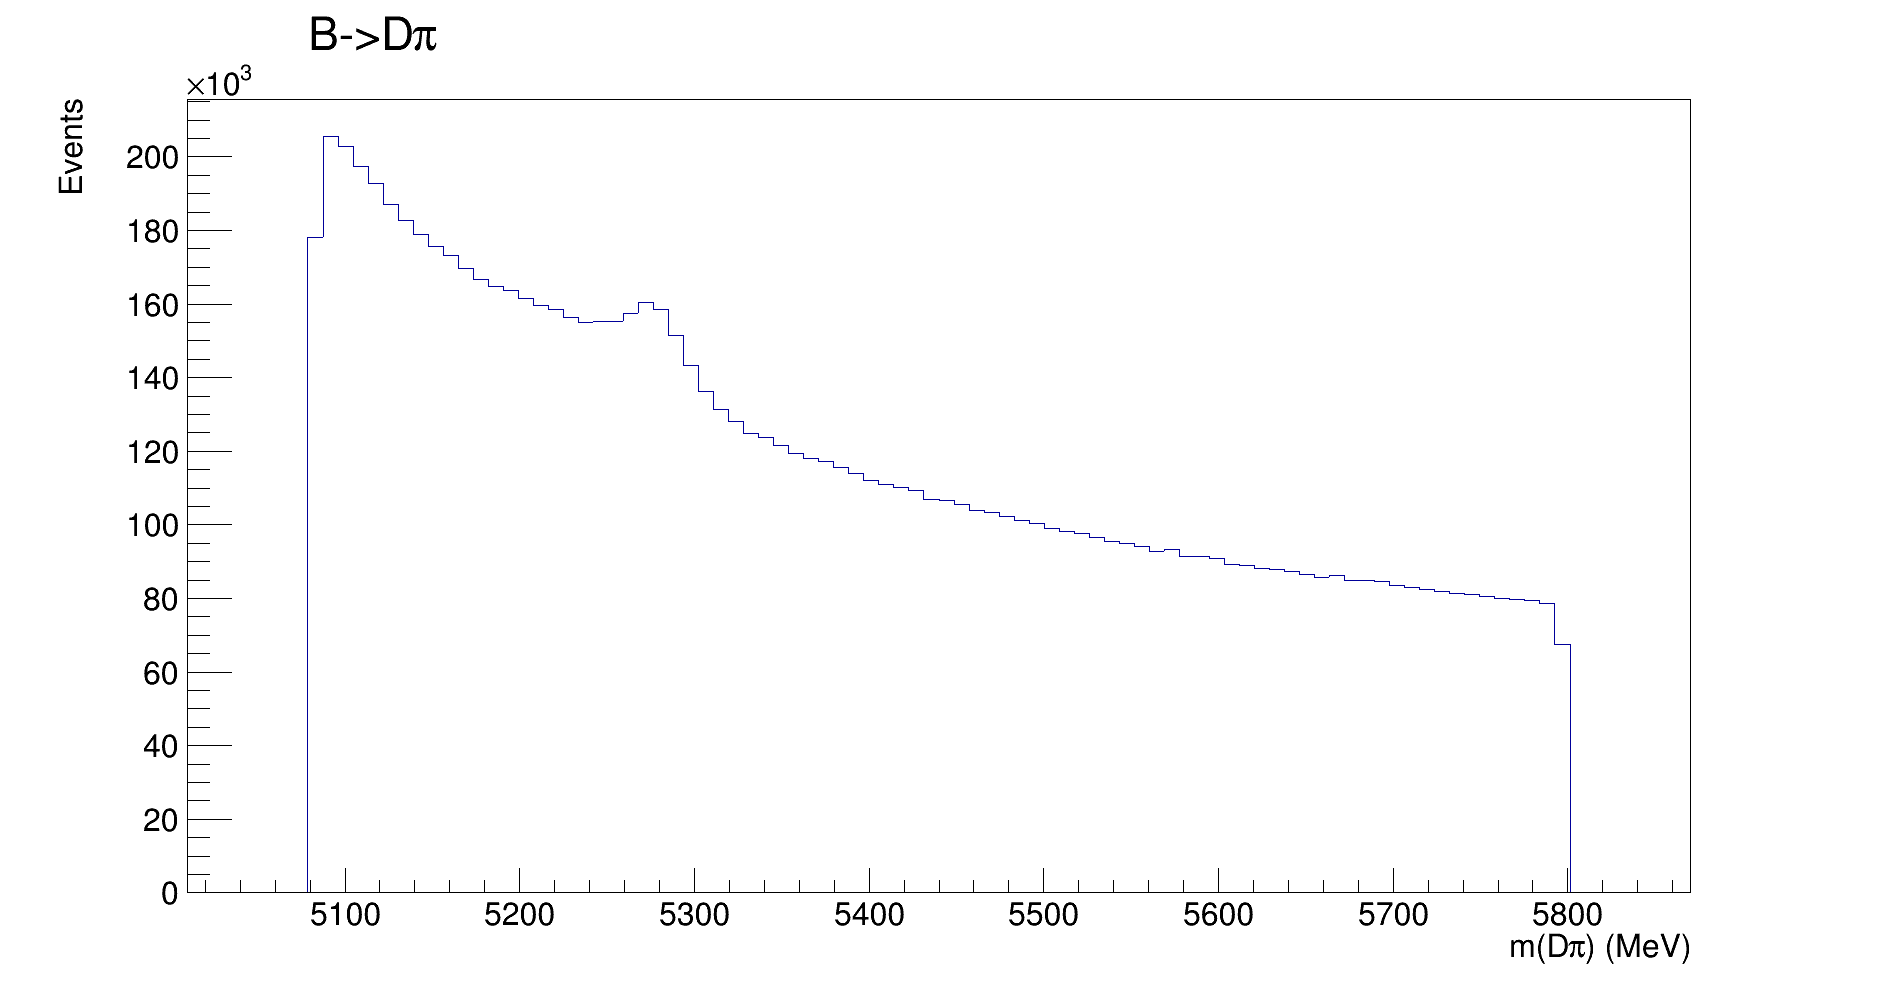
\includegraphics[width = 1.0\textwidth]{BMassBeforeCutsB2DPi.png}
      \caption{$m(D\pi)$ distribution}
    \end{subfigure}%
    \begin{subfigure}{0.5\textwidth}
      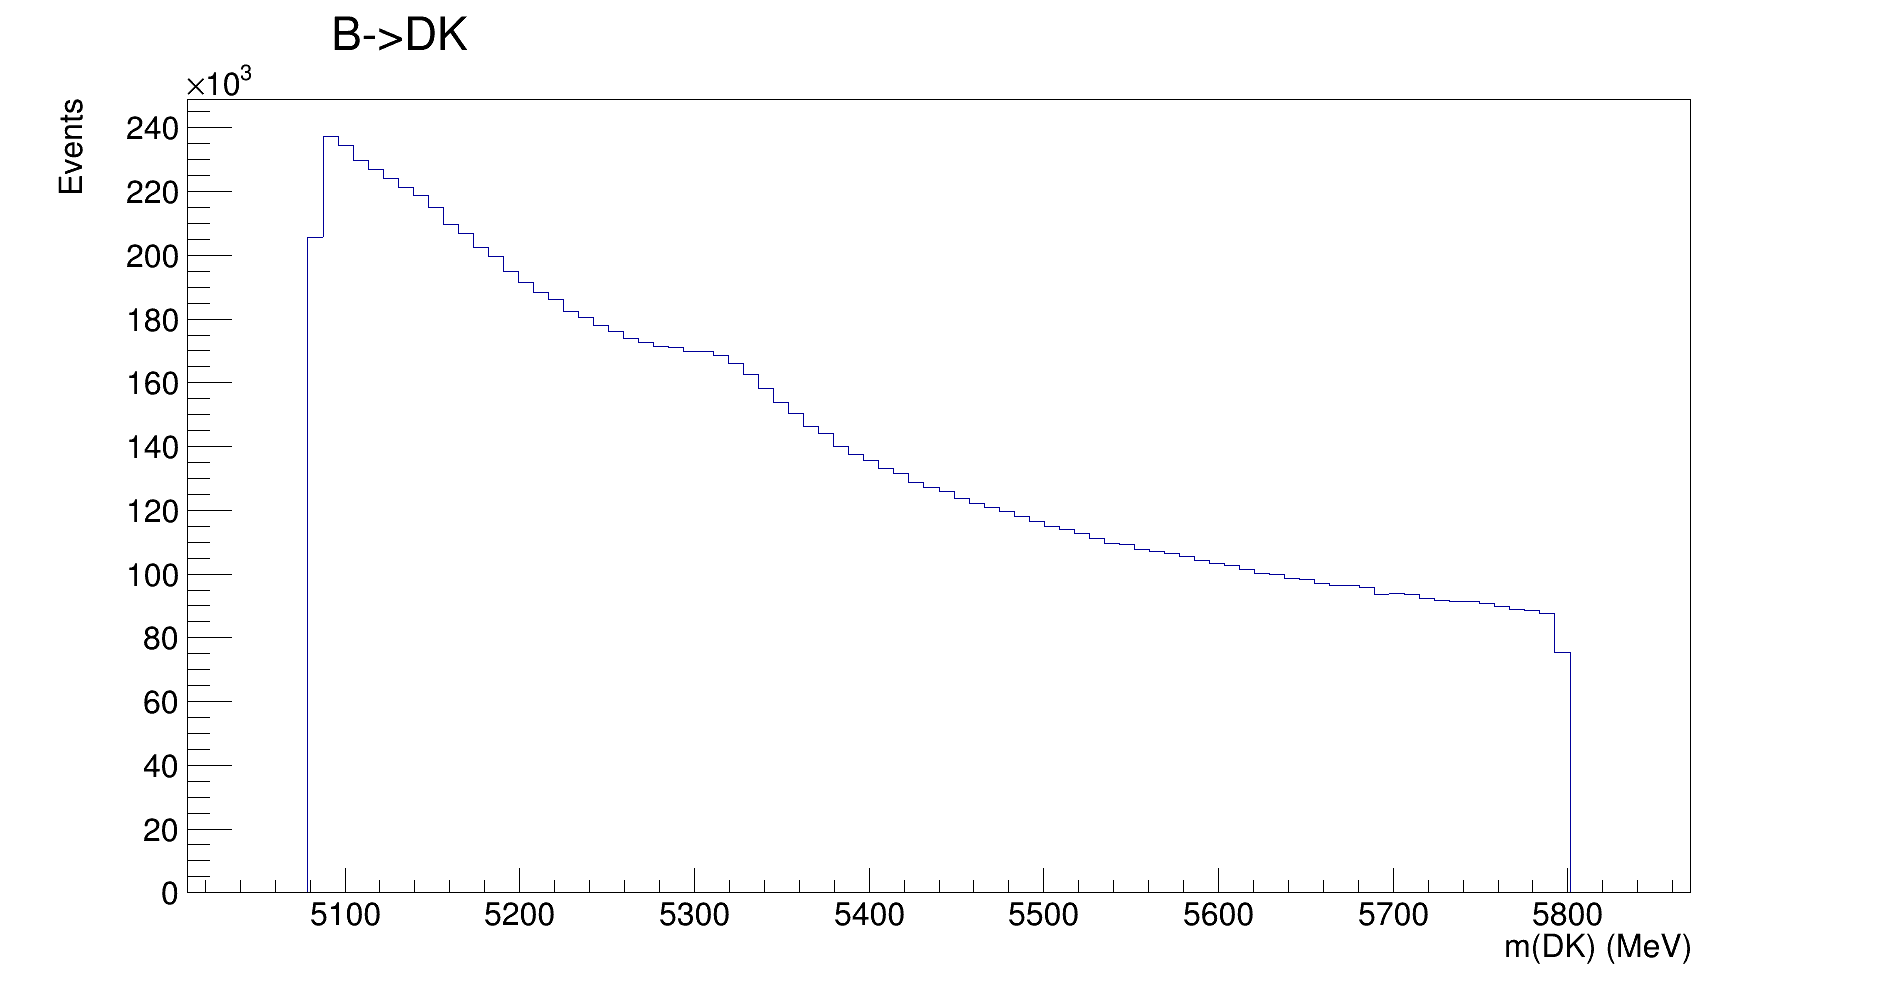
\includegraphics[width = 1.0\textwidth]{BMassBeforeCutsB2DK.png}
      \caption{$m(DK)$ distribution}
    \end{subfigure}
  \end{figure}
\end{frame}

\begin{frame}{BDT sample preparation}
  \begin{itemize}
    \setlength\itemsep{1.3em}
    \item{Signal training sample: $B\to D\pi$ MC samples}
    \item{Background training sample: High mass sideband in data}
    \begin{itemize}
      \item{$\SI{5800}{\mega\eV} < m(Dh) < \SI{7000}{\mega\eV}$}
    \end{itemize}
    \item{Signal region: $\SI{5080}{\mega\eV} < m(Dh) < \SI{5800}{\mega\eV}$}
    \item{Initial cuts:}
    \begin{itemize}
      \item{Standard trigger requirements}
      \item{Bachelor $P < \SI{100}{\giga\eV}$ and has RICH}
      \item{$K^\pm$ daughters $P < \SI{100}{\giga\eV}$ and has RICH}
      \item{DecayTreeFitter convergence}
      \item{$\abs{m(D) - m_\text{PDG}(D)} < \SI{25}{\mega\eV}$}
    \end{itemize}
  \end{itemize}
\end{frame}

\begin{frame}{BDT training}
    \begin{figure}
    \centering
    \vspace{-0.2cm}
    \begin{subfigure}{0.5\textwidth}
      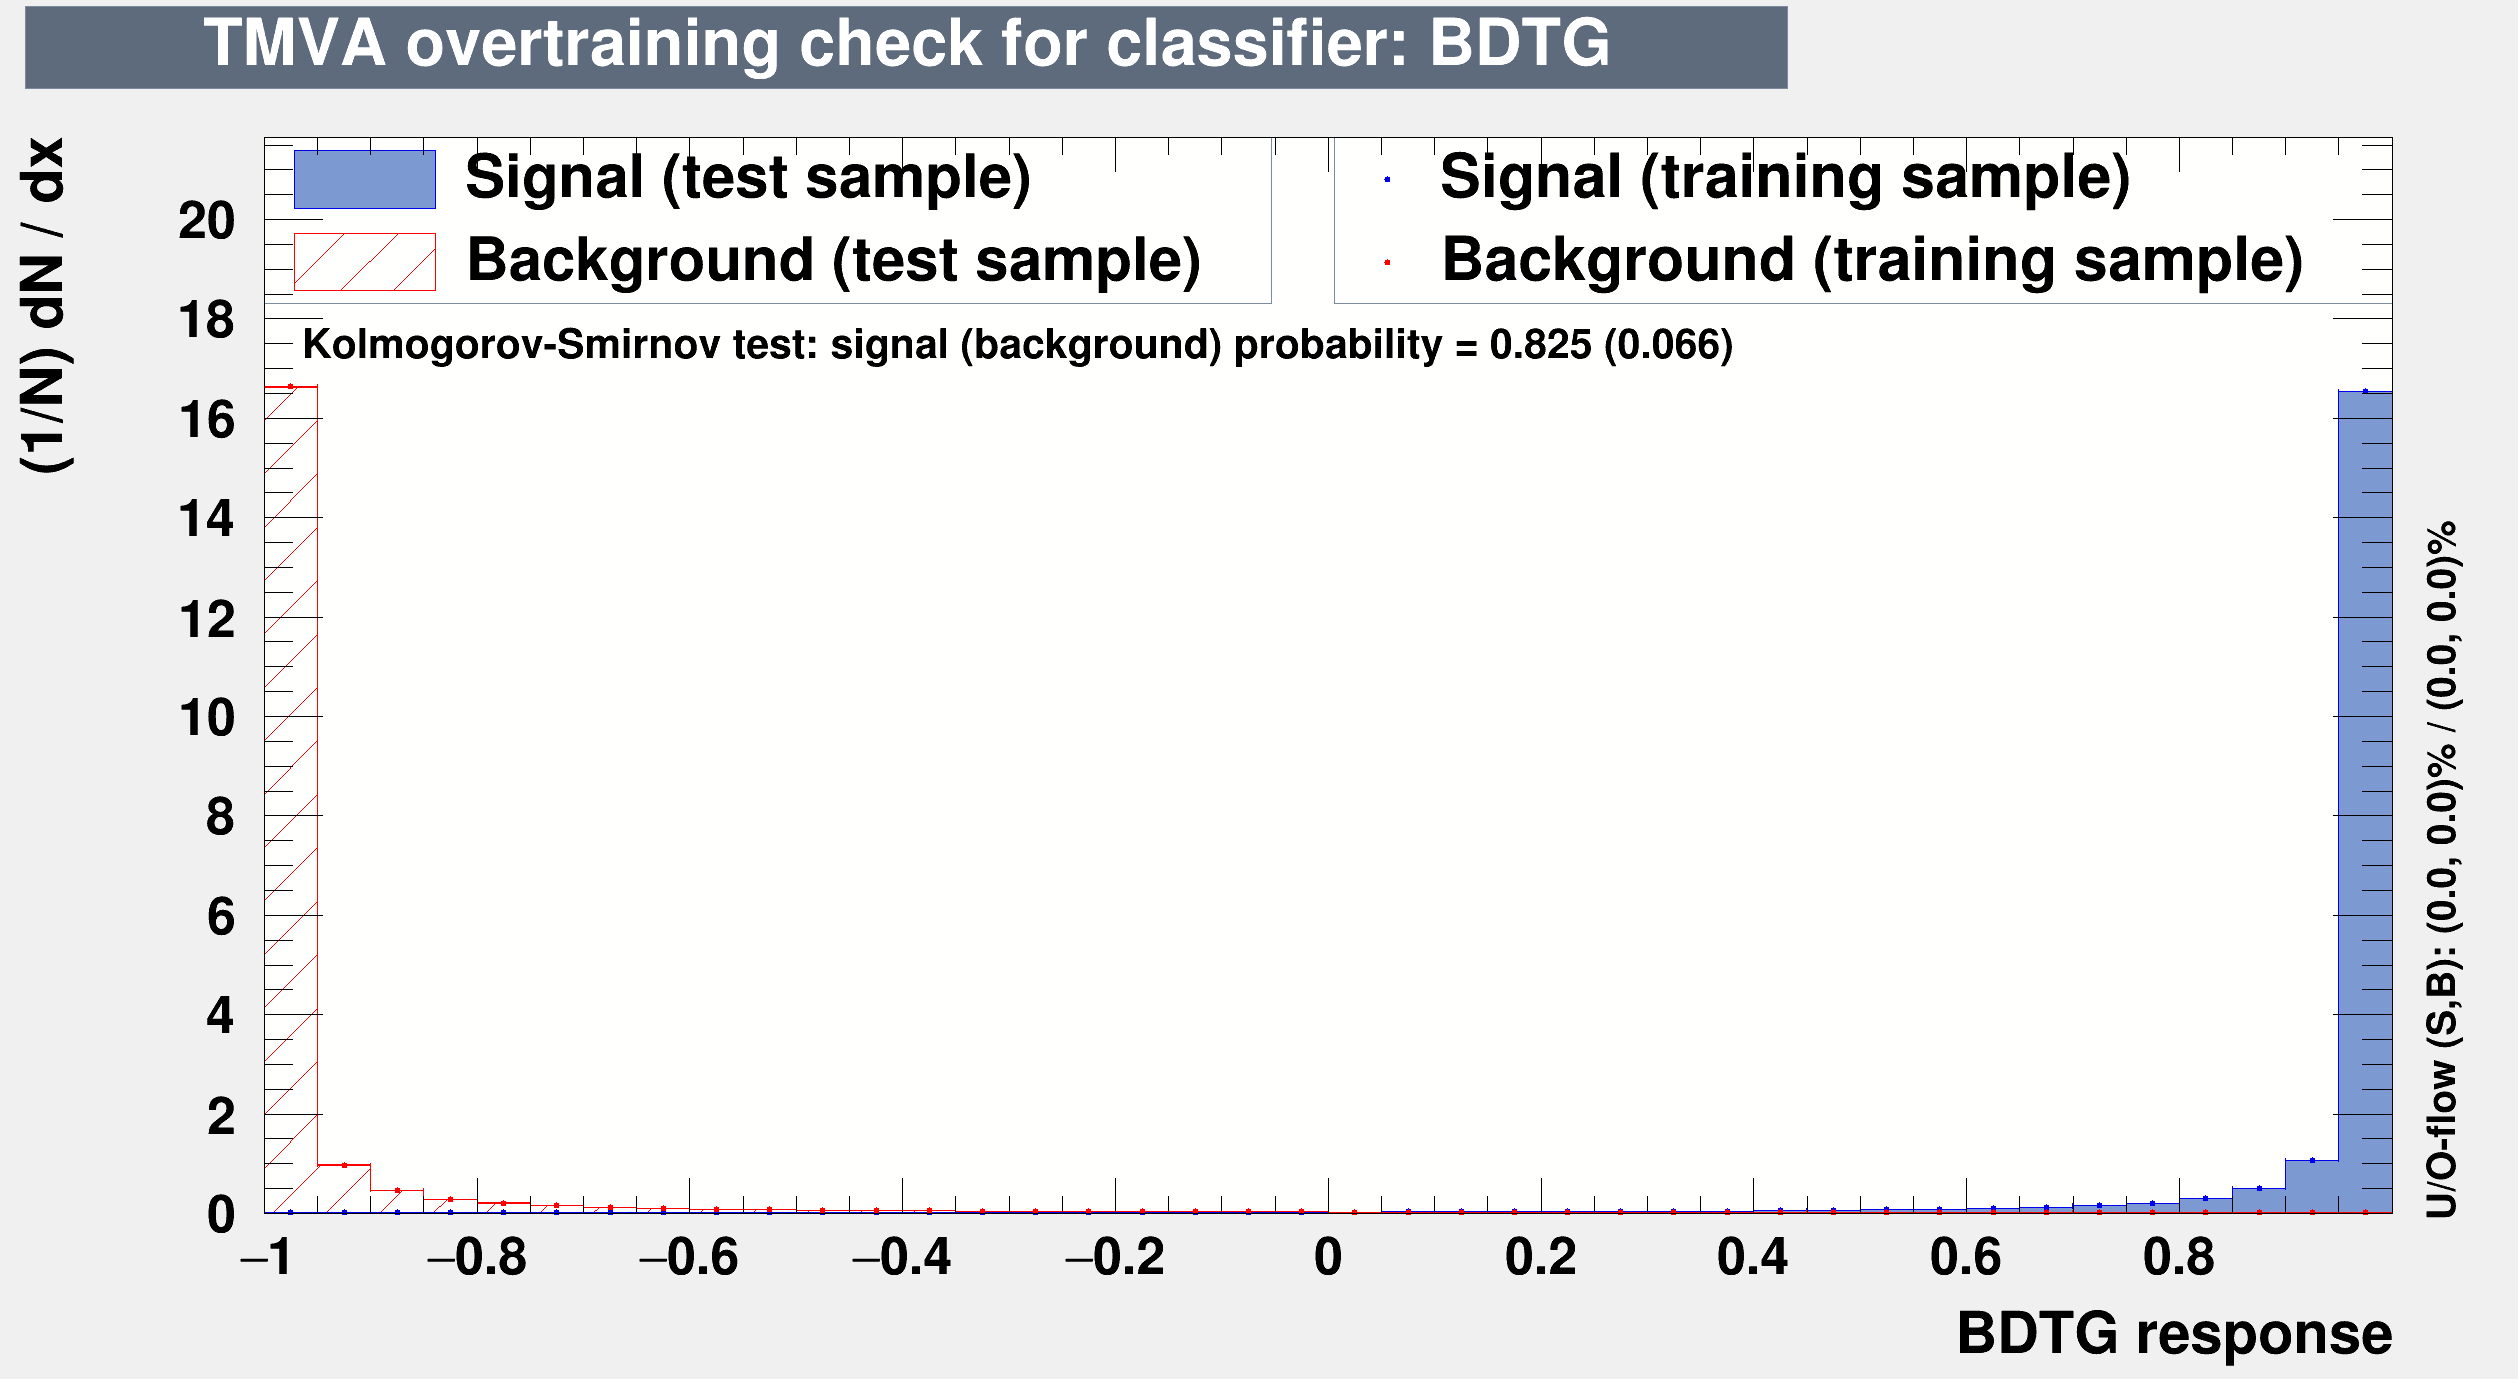
\includegraphics[width = 1.0\textwidth]{BDToutput.png}
      \caption{BDT output}
    \end{subfigure}%
    \begin{subfigure}{0.5\textwidth}
      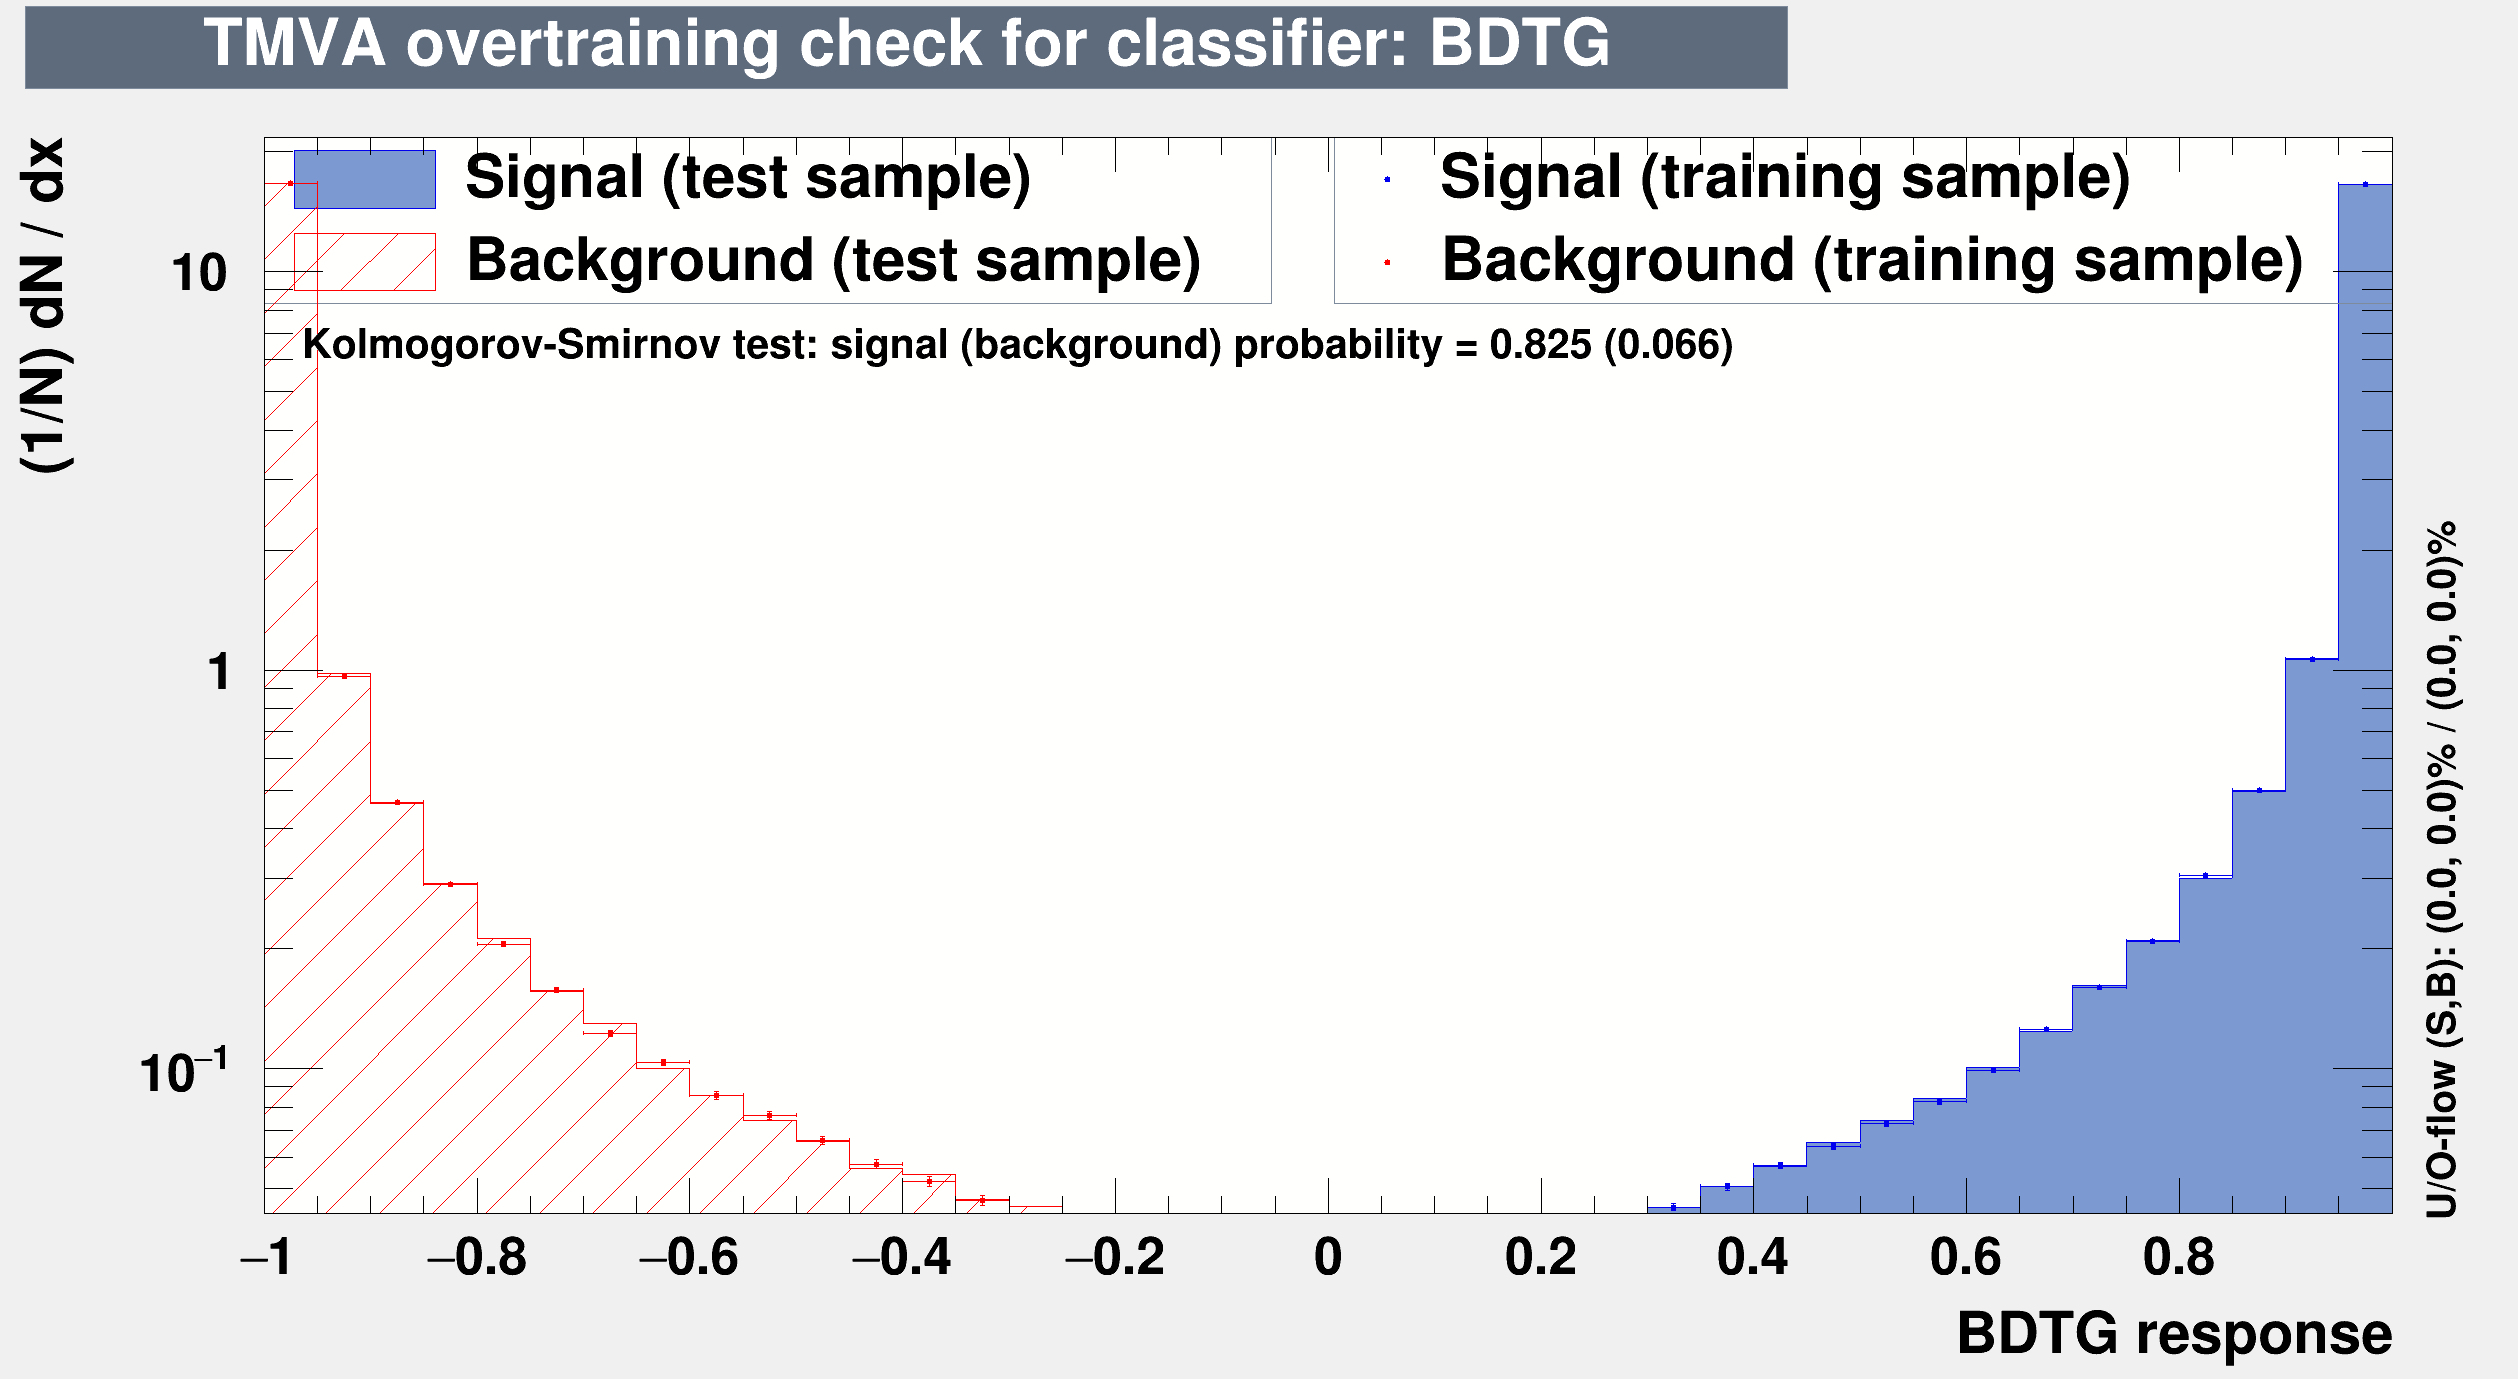
\includegraphics[width = 1.0\textwidth]{BDToutputLog.png}
      \caption{BDT output on a logarithmic scale}
    \end{subfigure}
  \end{figure}
\end{frame}

\begin{frame}{Final selection}
  \begin{itemize}
    \setlength\itemsep{1.3em}
    \item{PID cut for bachelor at $4$}
    \begin{itemize}
      \item{$\text{Bach\_PIDK} > 4$ for $B\to DK$}
      \item{$\text{Bach\_PIDK} < 4$ for $B\to D\pi$}
    \end{itemize}
    \item{$K^\pm$ daughter PID cut at $-5$}
    \item{DecayTreeFitter $\ln(\chi^2) < 3$}
    \item{$B$-$D$ flight significance at $0.5$}
    \item{BDT working point at $0.75$}
    \item{\textbf{Not} optimized yet}
  \end{itemize}
\end{frame}

\begin{frame}{Mass plots after final selection}
  \begin{figure}
    \centering
    \vspace{-0.2cm}
    \begin{subfigure}{0.5\textwidth}
      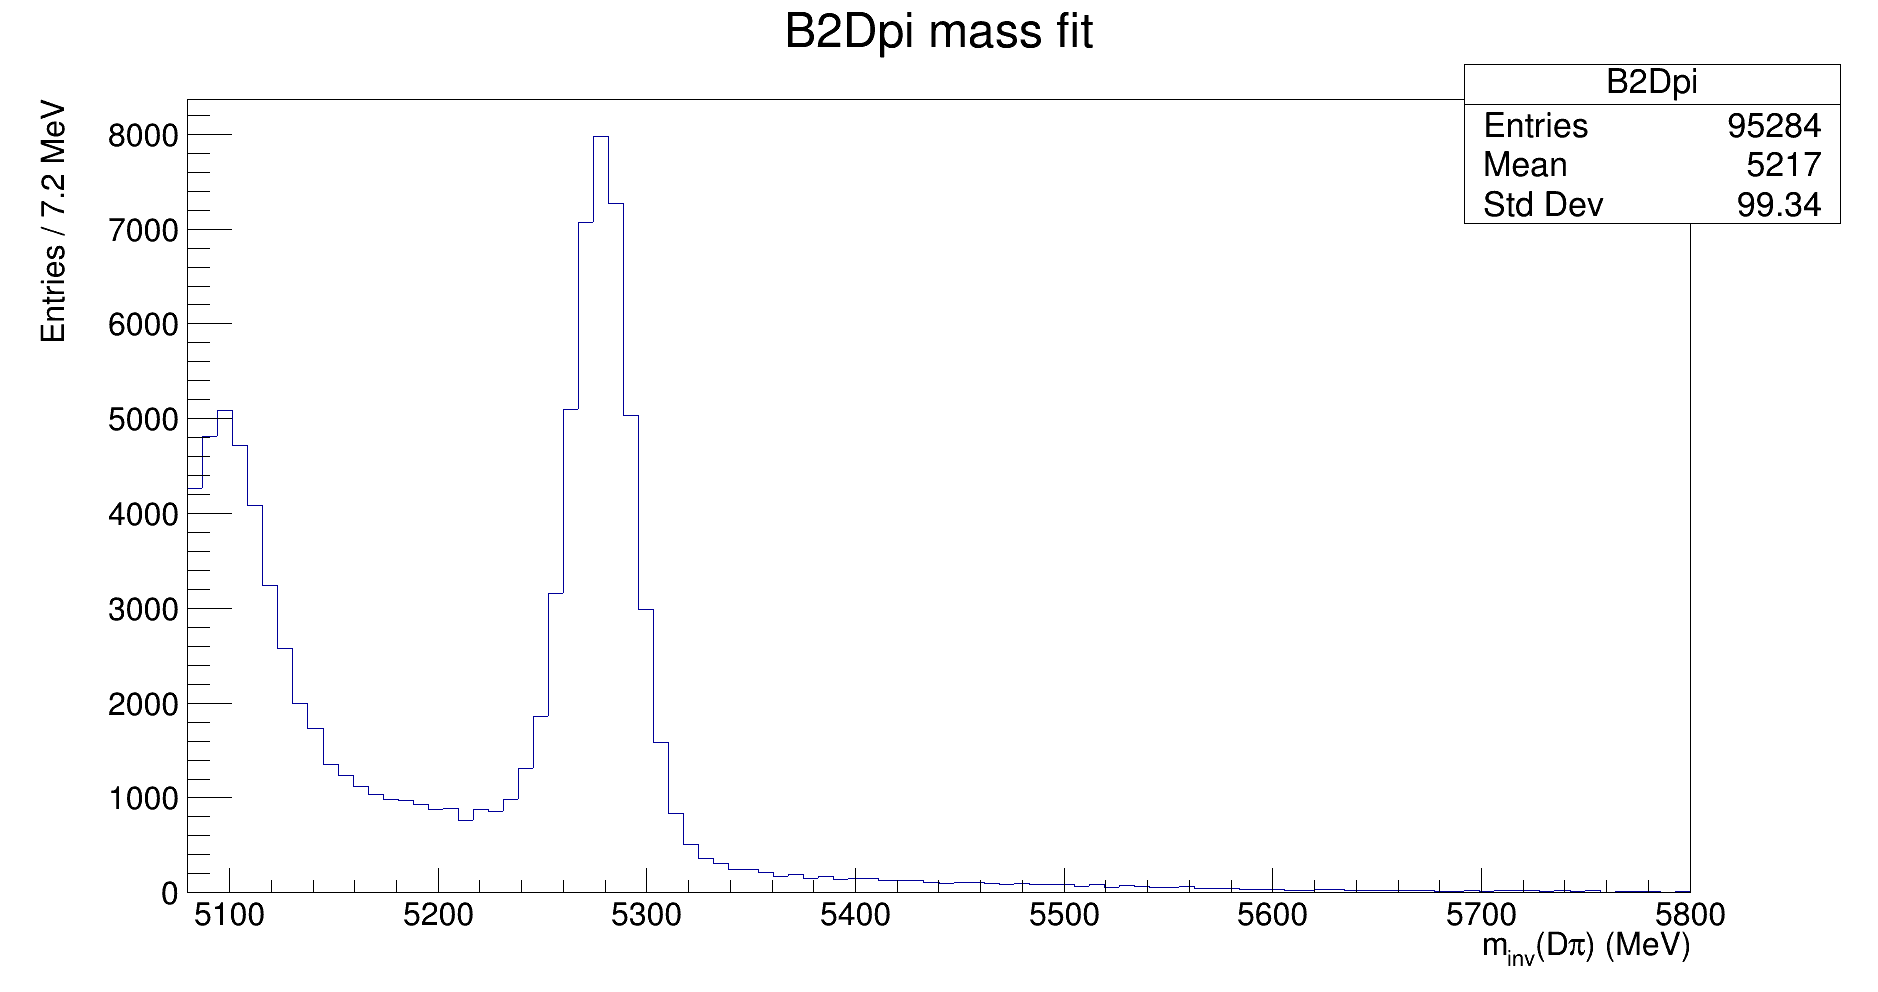
\includegraphics[width = 1.0\textwidth]{BMassAfterCutsB2DPi.png}
      \caption{$m(D\pi)$ distribution}
    \end{subfigure}%
    \begin{subfigure}{0.5\textwidth}
      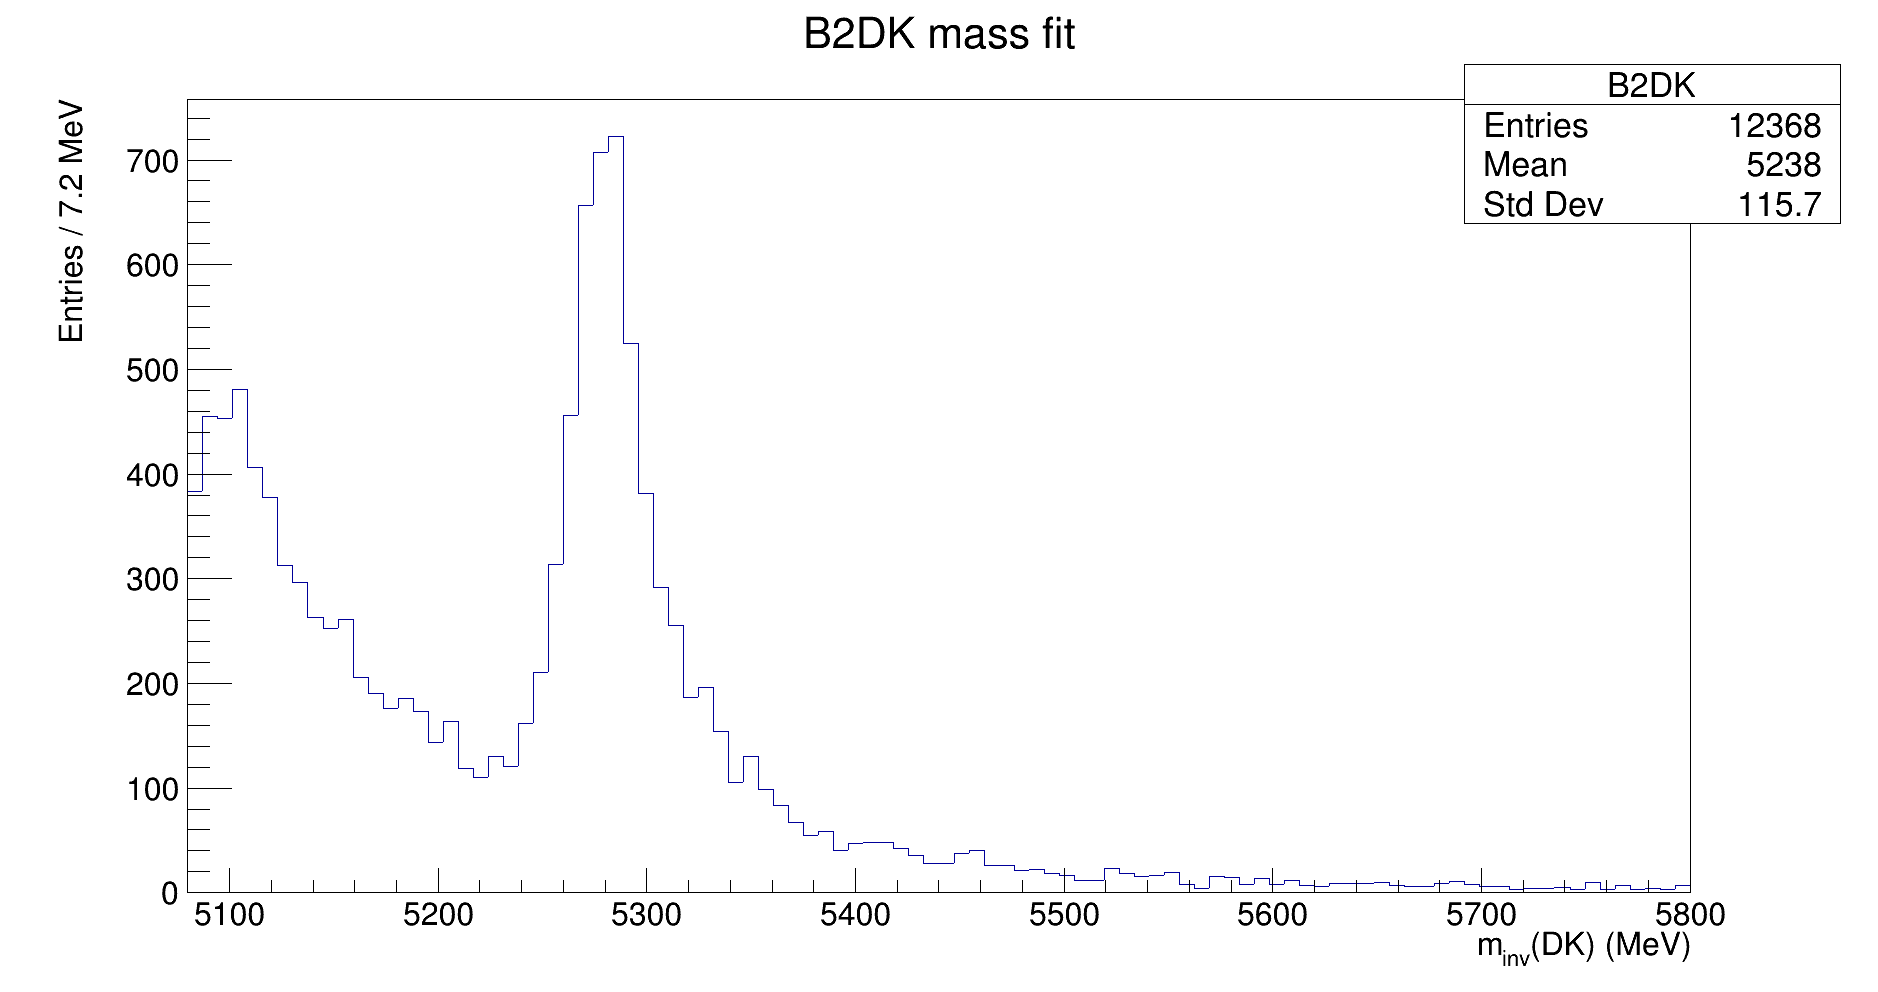
\includegraphics[width = 1.0\textwidth]{BMassAfterCutsB2DK.png}
      \caption{$m(DK)$ distribution}
    \end{subfigure}
  \end{figure}
\end{frame}

\begin{frame}{Mass fit}
  \begin{itemize}
    \item{Signal shape: Double Crystal Ball}
    \begin{itemize}
      \item{Tail parameters taken from fit to MC $B\to D\pi$}
      \item{Width and mean is floated}
    \end{itemize}
  \end{itemize}
  \begin{figure}
    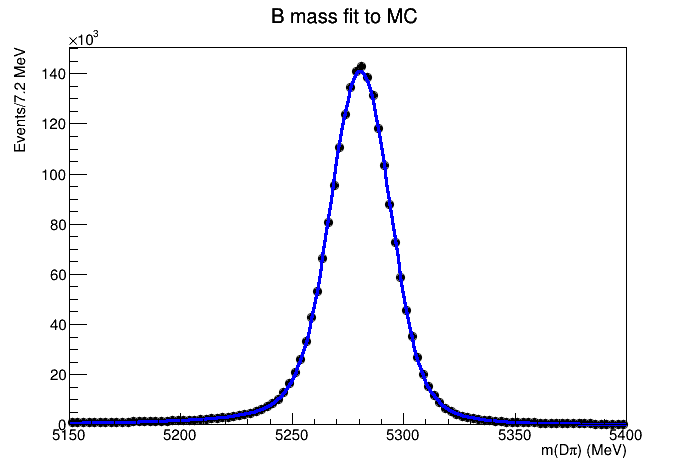
\includegraphics[width = 0.8\textwidth]{MassFitMC.png}
  \end{figure}
\end{frame}

\begin{frame}{Mass fit}
  \begin{itemize}
    \setlength\itemsep{1.3em}
    \item{Combinatorial background: Exponential curve}
    \item{Partially reconstructed background:}
    \begin{itemize}
      \item{Shape parameters taken from LHCb-ANA-2017-057.1}
      \item{$B^\pm\to(D^{*0}\to D^0[\pi^0])\pi^\pm$: HORNSdini}
      \item{$B^0\to(D^{*\pm}\to D^0[\pi^\mp])\pi^\pm$: HORNSdini}
      \item{$B^\pm\to D^0\to(\rho^\pm\to\pi^\pm[\pi^0])\pi^\pm$: HORNSdini}
      \item{$B^\pm\to(D^{*0}\to D^0[\gamma])\pi^\pm$: HILLdini}
    \end{itemize}
    \item{Further complication for $B\to DK$ mode:}
    \begin{itemize}
      \item{Cross-feed from $B\to D\pi$: Double Crystal Ball with same tail parameters as signal for now}
      \item{Mis-ID of partially reconstructed background: Haven't considered yet, absorb into a Gaussian for now}
    \end{itemize}
  \end{itemize}
\end{frame}

\begin{frame}{Mass fit plots}
  \begin{figure}
    \centering
    \vspace{-0.2cm}
    \begin{subfigure}{0.5\textwidth}
      \begin{overpic}[scale = 0.25, percent]{MassFitB2Dpi.png}
        \put(40, 50){\tiny Signal events: $43217 \pm 223$}
      \end{overpic}
      \caption{$m(D\pi)$ mass fit}
    \end{subfigure}%
    \begin{subfigure}{0.5\textwidth}
      \begin{overpic}[scale = 0.25, percent]{MassFitB2DK.png}
        \put(40, 50){\tiny Signal events: $3596 \pm 137$}
      \end{overpic}
      \caption{$m(DK)$ mass fit}
    \end{subfigure}
  \end{figure}
  \begin{itemize}
    \color{red}
    \item{Signal}
    \color{green}
    \item{Partially reconstructed background}
    \color{blue}
    \item{Combinatorial background (dashed)}
    \color{cyan}
    \item{Cross feed}
    \color{black}
    \item{Mis-ID of partially reconstructed background}
  \end{itemize}
\end{frame}


% \section{Binned fit of \texorpdfstring{$D\to K^+K^-\pi^+\pi^-$}{D to K+K-pi+pi-}}
% \begin{frame}{Binned fit of $D\to K^+K^-\pi^+\pi^-$}
%   \vspace{-0.5cm}
%   \begin{align*}
%     \mathcal{A}(B^-\to(K^+K^-\pi^+\pi^-)_DK^-) =& \mathcal{A}_B\mathcal{A}(D^0\to K^+K^-\pi^+\pi^-) \\
%   +& \mathcal{A}_B\mathcal{A}(\bar{D^0}\to K^+K^-\pi^+\pi^-)r_Be^{i(\delta_B - \gamma)}
%   \end{align*}
%   \vspace{-0.5cm}
%   \begin{block}{Event yield in bin $i$}
%     $N^-_i = h_{B^-}\Big(K_i + \big(x_-^2 + y_-^2\big)\bar{K_i} + 2\sqrt{K_i\bar{K_i}}\big(x_-c_i + y_-s_i\big)\Big)$
%     $N^+_i = h_{B^+}\Big(\bar{K_i} + \big(x_+^2 + y_+^2\big)K_i + 2\sqrt{K_i\bar{K_i}}\big(x_+c_i - y_+s_i\big)\Big)$
%   \end{block}
%   \begin{block}{CP-violating observables}
%     $x_\pm = r_B\cos(\delta_B\pm\gamma), \quad y_\pm = r_B\sin(\delta_B\pm\gamma)$
%   \end{block}
%   \begin{itemize}
%     \item{$c_i$, $s_i$: Amplitude-averaged strong phase difference of $D$ decay}
%     \item{Measure $c_i$ and $s_i$ at BES III detector}
%     \item{Can measure $K_i$ and $\bar{K_i}$ at both LHCb and BES III}
%     \item{Need to divide phase space into bins}
%   \end{itemize}
% \end{frame}

% \begin{frame}{Pull studies}
%   \begin{itemize}
%     \item{Pull studies shows that this works}
%     \item{Used an arbitrary and naive binning scheme with $4$ bins}
%     \item{$x_\pm$ pulls show asymmetric tails for $\SI{2e3}{}$ events}
%     \item{$x_\pm$ and $y_\pm$ are all satisfactory for $\SI{2e4}{}$ events}
%   \end{itemize}
%   \begin{block}{Naive binning scheme}
%     Split phase space along the boundaries $E_{K^+} = E_{K_-}$ and $E_{\pi^+} = E_{\pi^-}$ \\
%     Bin $1$: $E_{K^+} > E_{K^-}, \quad E_{\pi^+} > E_{\pi^-}$, \dots
%   \end{block}
%   \begin{block}{$D$ decay hadronic parameters}
%     \begin{equation*}
%       c_i = \frac{\int_i\dd{\Phi}|\mathcal{A}(D^0)||\mathcal{A}(\bar{D^0})|\cos(\delta_D)}{\sqrt{\int_i\dd{\Phi}\abs{\mathcal{A}(D^0)}^2\int_i\dd{\Phi}\abs{\mathcal{A}(D^0)}^2}}, \quad K_i = \frac{\int_i\dd{\Phi}|\mathcal{A}(D^0)|^2}{\sum_j\int_j\dd{\Phi}\abs{\mathcal{A}(D^0)}^2}
%     \end{equation*}
%   \end{block}
% \end{frame}

% \begin{frame}{Pull study with $\SI{2e3}{}$ events}
%   \begin{figure}
%     \centering
%     \vspace{-0.2cm}
%     \begin{subfigure}{0.5\textwidth}
%       \includegraphics[width = 1.0\textwidth]{xplus1K1K.png}
%       \caption{$x_+$ pull}
%     \end{subfigure}%
%     \begin{subfigure}{0.5\textwidth}
%       \includegraphics[width = 1.0\textwidth]{xminus1K1K.png}
%       \caption{$x_-$ pull}
%     \end{subfigure}
%     \begin{subfigure}{0.5\textwidth}
%       \includegraphics[width = 1.0\textwidth]{yplus1K1K.png}
%       \caption{$y_+$ pull}
%     \end{subfigure}%
%     \begin{subfigure}{0.5\textwidth}
%       \includegraphics[width = 1.0\textwidth]{yminus1K1K.png}
%       \caption{$y_-$ pull}
%     \end{subfigure}
%   \end{figure}
% \end{frame}

\begin{frame}{Backup slides}
  \begin{center}
    DaVinci error message:
  \end{center}
  \begin{figure}
    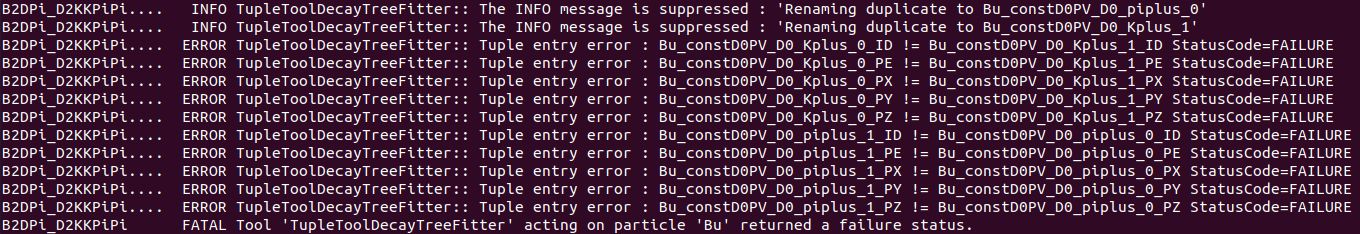
\includegraphics[width = 1\textwidth]{DaVinciError.png}
  \end{figure}
\end{frame}

\end{document}
